% Options for packages loaded elsewhere
\PassOptionsToPackage{unicode}{hyperref}
\PassOptionsToPackage{hyphens}{url}
%
\documentclass[
]{article}
\title{STA 137 Final Project}
\author{Camden Possinger}
\date{2022-06-05}

\usepackage{amsmath,amssymb}
\usepackage{lmodern}
\usepackage{iftex}
\ifPDFTeX
  \usepackage[T1]{fontenc}
  \usepackage[utf8]{inputenc}
  \usepackage{textcomp} % provide euro and other symbols
\else % if luatex or xetex
  \usepackage{unicode-math}
  \defaultfontfeatures{Scale=MatchLowercase}
  \defaultfontfeatures[\rmfamily]{Ligatures=TeX,Scale=1}
\fi
% Use upquote if available, for straight quotes in verbatim environments
\IfFileExists{upquote.sty}{\usepackage{upquote}}{}
\IfFileExists{microtype.sty}{% use microtype if available
  \usepackage[]{microtype}
  \UseMicrotypeSet[protrusion]{basicmath} % disable protrusion for tt fonts
}{}
\makeatletter
\@ifundefined{KOMAClassName}{% if non-KOMA class
  \IfFileExists{parskip.sty}{%
    \usepackage{parskip}
  }{% else
    \setlength{\parindent}{0pt}
    \setlength{\parskip}{6pt plus 2pt minus 1pt}}
}{% if KOMA class
  \KOMAoptions{parskip=half}}
\makeatother
\usepackage{xcolor}
\IfFileExists{xurl.sty}{\usepackage{xurl}}{} % add URL line breaks if available
\IfFileExists{bookmark.sty}{\usepackage{bookmark}}{\usepackage{hyperref}}
\hypersetup{
  pdftitle={STA 137 Final Project},
  pdfauthor={Camden Possinger},
  hidelinks,
  pdfcreator={LaTeX via pandoc}}
\urlstyle{same} % disable monospaced font for URLs
\usepackage[margin=1in]{geometry}
\usepackage{color}
\usepackage{fancyvrb}
\newcommand{\VerbBar}{|}
\newcommand{\VERB}{\Verb[commandchars=\\\{\}]}
\DefineVerbatimEnvironment{Highlighting}{Verbatim}{commandchars=\\\{\}}
% Add ',fontsize=\small' for more characters per line
\usepackage{framed}
\definecolor{shadecolor}{RGB}{248,248,248}
\newenvironment{Shaded}{\begin{snugshade}}{\end{snugshade}}
\newcommand{\AlertTok}[1]{\textcolor[rgb]{0.94,0.16,0.16}{#1}}
\newcommand{\AnnotationTok}[1]{\textcolor[rgb]{0.56,0.35,0.01}{\textbf{\textit{#1}}}}
\newcommand{\AttributeTok}[1]{\textcolor[rgb]{0.77,0.63,0.00}{#1}}
\newcommand{\BaseNTok}[1]{\textcolor[rgb]{0.00,0.00,0.81}{#1}}
\newcommand{\BuiltInTok}[1]{#1}
\newcommand{\CharTok}[1]{\textcolor[rgb]{0.31,0.60,0.02}{#1}}
\newcommand{\CommentTok}[1]{\textcolor[rgb]{0.56,0.35,0.01}{\textit{#1}}}
\newcommand{\CommentVarTok}[1]{\textcolor[rgb]{0.56,0.35,0.01}{\textbf{\textit{#1}}}}
\newcommand{\ConstantTok}[1]{\textcolor[rgb]{0.00,0.00,0.00}{#1}}
\newcommand{\ControlFlowTok}[1]{\textcolor[rgb]{0.13,0.29,0.53}{\textbf{#1}}}
\newcommand{\DataTypeTok}[1]{\textcolor[rgb]{0.13,0.29,0.53}{#1}}
\newcommand{\DecValTok}[1]{\textcolor[rgb]{0.00,0.00,0.81}{#1}}
\newcommand{\DocumentationTok}[1]{\textcolor[rgb]{0.56,0.35,0.01}{\textbf{\textit{#1}}}}
\newcommand{\ErrorTok}[1]{\textcolor[rgb]{0.64,0.00,0.00}{\textbf{#1}}}
\newcommand{\ExtensionTok}[1]{#1}
\newcommand{\FloatTok}[1]{\textcolor[rgb]{0.00,0.00,0.81}{#1}}
\newcommand{\FunctionTok}[1]{\textcolor[rgb]{0.00,0.00,0.00}{#1}}
\newcommand{\ImportTok}[1]{#1}
\newcommand{\InformationTok}[1]{\textcolor[rgb]{0.56,0.35,0.01}{\textbf{\textit{#1}}}}
\newcommand{\KeywordTok}[1]{\textcolor[rgb]{0.13,0.29,0.53}{\textbf{#1}}}
\newcommand{\NormalTok}[1]{#1}
\newcommand{\OperatorTok}[1]{\textcolor[rgb]{0.81,0.36,0.00}{\textbf{#1}}}
\newcommand{\OtherTok}[1]{\textcolor[rgb]{0.56,0.35,0.01}{#1}}
\newcommand{\PreprocessorTok}[1]{\textcolor[rgb]{0.56,0.35,0.01}{\textit{#1}}}
\newcommand{\RegionMarkerTok}[1]{#1}
\newcommand{\SpecialCharTok}[1]{\textcolor[rgb]{0.00,0.00,0.00}{#1}}
\newcommand{\SpecialStringTok}[1]{\textcolor[rgb]{0.31,0.60,0.02}{#1}}
\newcommand{\StringTok}[1]{\textcolor[rgb]{0.31,0.60,0.02}{#1}}
\newcommand{\VariableTok}[1]{\textcolor[rgb]{0.00,0.00,0.00}{#1}}
\newcommand{\VerbatimStringTok}[1]{\textcolor[rgb]{0.31,0.60,0.02}{#1}}
\newcommand{\WarningTok}[1]{\textcolor[rgb]{0.56,0.35,0.01}{\textbf{\textit{#1}}}}
\usepackage{graphicx}
\makeatletter
\def\maxwidth{\ifdim\Gin@nat@width>\linewidth\linewidth\else\Gin@nat@width\fi}
\def\maxheight{\ifdim\Gin@nat@height>\textheight\textheight\else\Gin@nat@height\fi}
\makeatother
% Scale images if necessary, so that they will not overflow the page
% margins by default, and it is still possible to overwrite the defaults
% using explicit options in \includegraphics[width, height, ...]{}
\setkeys{Gin}{width=\maxwidth,height=\maxheight,keepaspectratio}
% Set default figure placement to htbp
\makeatletter
\def\fps@figure{htbp}
\makeatother
\setlength{\emergencystretch}{3em} % prevent overfull lines
\providecommand{\tightlist}{%
  \setlength{\itemsep}{0pt}\setlength{\parskip}{0pt}}
\setcounter{secnumdepth}{-\maxdimen} % remove section numbering
\usepackage{booktabs}
\usepackage{longtable}
\usepackage{array}
\usepackage{multirow}
\usepackage{wrapfig}
\usepackage{float}
\usepackage{colortbl}
\usepackage{pdflscape}
\usepackage{tabu}
\usepackage{threeparttable}
\usepackage{threeparttablex}
\usepackage[normalem]{ulem}
\usepackage{makecell}
\usepackage{xcolor}
\ifLuaTeX
  \usepackage{selnolig}  % disable illegal ligatures
\fi

\begin{document}
\maketitle

\hypertarget{introduction}{%
\subsubsection{Introduction}\label{introduction}}

The Central African Republic (C.A.R) is regarded as one of the most
underdeveloped countries in the world ranking 188 out of 189 on the
United Nations Human Development Index. The C.A.R was brought under
French colonial rule in the late 19th century and became independent in
1960. The French colonists favored certain ethnic groups over others
which resulted in political rivalries that still exist today. After the
C.A.R gained independence the country was plagued with political unrest
and interethnic civil war fueled by colonialism. After the C.A.R gained
independence the country lost most of its financial investment from
France and struggled to find other international financial backing. In
the 1990s the C.A.R's economy was strained due to a decrease in the
price of cash crops, inflated costs of imports, diamond smuggling, and
most significantly corruption and financial mismanagement. This economic
strain created a situation where the government was not able to pay the
salaries of their military and the entire public sector which created
major political unrest that continues today. The country's economy
mainly consists of agriculture, mining diamonds, and timber, but is
hindered by a poor transportation network. There are no railroads and
only 400 miles of paved roads in the country so most commerce is
transported by various rivers to the Congo. In this data analysis, we
will explore and model global export data from the Central African
Republic from when the country gained independence in 1960 to 2017.

\hypertarget{exploratory-data-analysis}{%
\subsubsection{Exploratory Data
Analysis}\label{exploratory-data-analysis}}

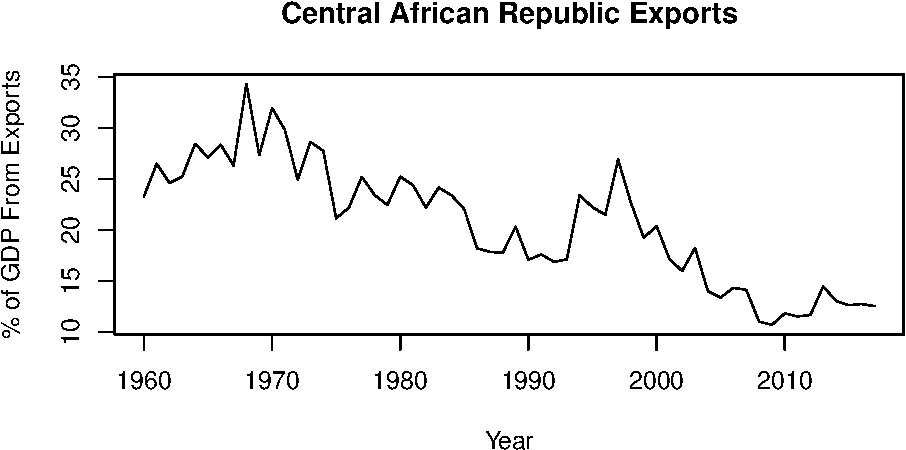
\includegraphics{STA_137_Final_Project_files/figure-latex/unnamed-chunk-2-1.pdf}

The above plot shows the C.A.R's percentage of GDP from exports over the
course of 57 years from 1960 to 2017. In this plot we can see a clear
overall downward trend over time with some periods of growth in the late
1960s and 1990s. We can see that the average of this data is not
constant so it is not stationary which is required for a formal
statistical analysis of this data. To combat this issue we must
transform our data to create a stationary time series.

\hypertarget{data-transformation}{%
\subsubsection{Data Transformation}\label{data-transformation}}

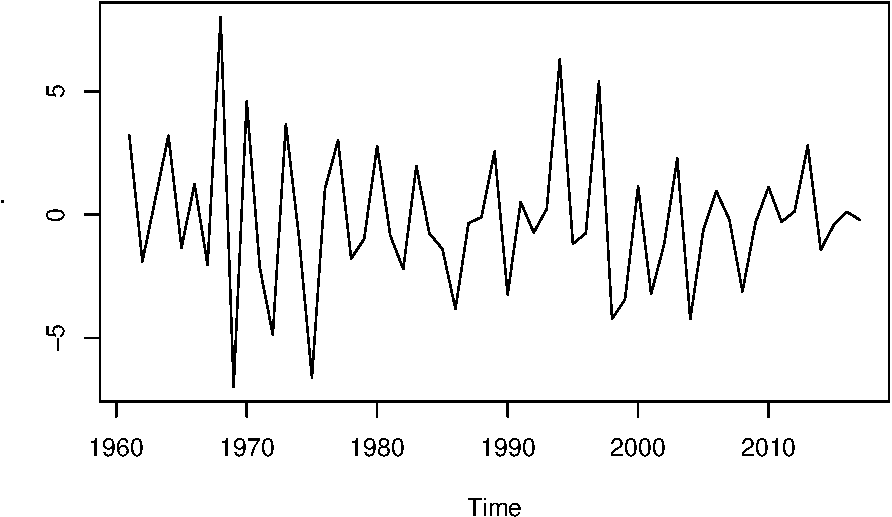
\includegraphics{STA_137_Final_Project_files/figure-latex/unnamed-chunk-3-1.pdf}

In this plot the first order difference of \(x_t\) which is the original
C.A.R export data. We define the first order difference of \(x_t\) as:

\[\Delta x_t = x_t - x_{t-1}\]

This differencing creates a stationary time series with mean close to 0
that we can potentially model.

\begin{center}

\begin{tabular}{c}
\hline
Mean\\
\hline
-0.1886778\\
\hline
\end{tabular}
\end{center}

Now let's look at the Autocorrelation Function (ACF) and Partial
Autocorrlation Function (PACF) of this data to see if there are any
relationships between observed data points based on the lagged time
between them to get an idea of what type of model will fit best.

\hypertarget{acfpacf}{%
\subsubsection{ACF/PACF}\label{acfpacf}}

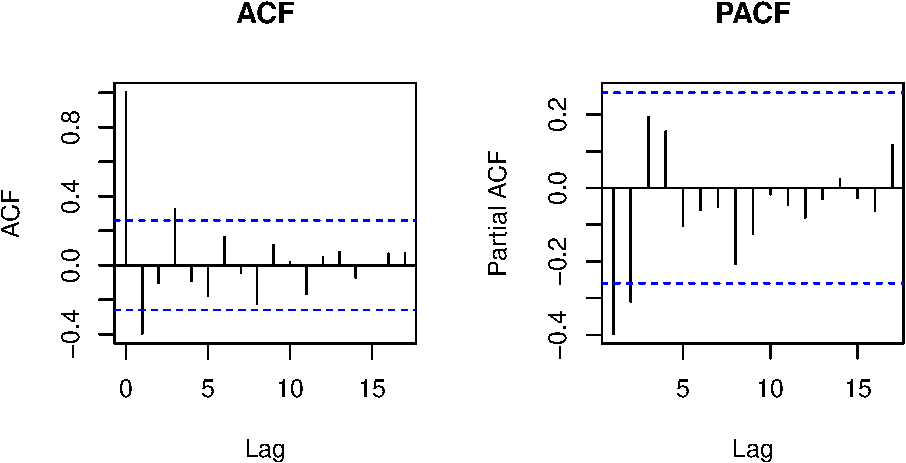
\includegraphics{STA_137_Final_Project_files/figure-latex/unnamed-chunk-5-1.pdf}

Here we have the plots for both the ACF and PACF for our differenced
C.A.R export data. Each lag indicates the distance between any two
observed data points. For example if the lag is 2 then the ACF reports
the Autocorrelation between \(x_1\) and \(x_3\) or \(x_5\) and \(x_7\).
The PACF follows the same interpretation as the ACF but is calulated
differently. We can interpret this from the ACF/PACF plots because we
assume our time series data is stationary.

The ACF indicates that we should use a Moving Average model with one
previous data point defined as:

\begin{center}
If we set $\Delta x_t = y_t$ then: 
\end{center}

\[MA(1) = y_t =  \theta w_{t-1} + w_t\]

\begin{center}

where $\theta$ is an unknown parameter and $w_{t}$ is a random white noise process.

The PACF indicates that we should use an Autoregressive model with two previous data points defined as:
\[AR(2) = y_t = \phi_1 y_{t-1} + \phi_2 y_{t-2} + w_t\]

where $\phi_1,\phi_2$ are unknown parameters and $w_{t}$ is a random white noise process.


\end{center}

\hypertarget{modelling}{%
\subsubsection{Modelling}\label{modelling}}

Based on the ACF/PACF from the previous section we have identified two
models that have potential to be a good fit for our C.A.R. export data.
When interpreting and selecting a model we look for whether the
coefficients are significant, which model has the smallest AIC/BIC, and
whether the residuals are white noise.

\hypertarget{ma1}{%
\subsubsection{MA(1)}\label{ma1}}

First let's take a look at our fitted MA(1) model.

\begin{center}

\begin{tabular}{l|r|r|r|r}
\hline
  & Estimate & SE & t.value & p.value\\
\hline
ma1 & -0.4172 & 0.1042 & -4.0042 & 2e-04\\
\hline
\end{tabular}
\end{center}

In this table R conducts a one sample t test to determine if \(\theta\)
is 0 or not. This test is defined as:

\[H_0: \theta = 0  \] \[H_A: \theta \neq 0  \]

Since the p-value is small we can reject the null hypothesis and
conclude that \(\theta \neq 0\) We can also see that the estimate for
\(\theta\) is -0.4172 so our fitted model is:

\[y_t = (-0.4172) w_{t-1} + w_t\]

Now let's take a look at the residuals.

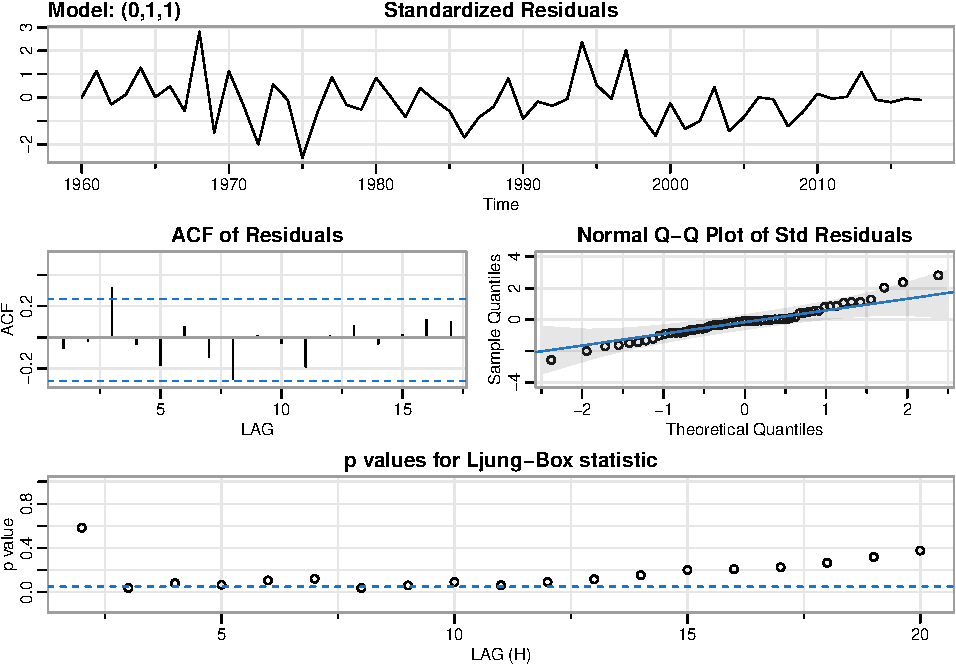
\includegraphics{STA_137_Final_Project_files/figure-latex/unnamed-chunk-8-1.pdf}

The main things to look for in the residuals is that their mean is 0 and
check to see if each residual is uncorrelated with all other residuals.
We can see from the Standardized Residuals plot that the mean seems to
be around 0 which satisfies our first property of white noise. However
the ACF and small p-values for the Ljung-Box Statistic show that the
residuals are correlated, so we cannot assume that the residuals are a
white noise process. The Ljung-Box test is defined as:

\begin{center}

$H_0 =$ The residuals are independently distributed \\
$H_A =$ The residuals are not independently distributed

\end{center}

\hypertarget{ar2}{%
\subsubsection{AR(2)}\label{ar2}}

Next let's take a look at our fitted AR(2) model.

\begin{center}

\begin{tabular}{l|r|r|r|r}
\hline
  & Estimate & SE & t.value & p.value\\
\hline
ar1 & -0.5050 & 0.1266 & -3.9889 & 0.0002\\
\hline
ar2 & -0.2897 & 0.1254 & -2.3101 & 0.0247\\
\hline
\end{tabular}
\end{center}

From this table we can conclude that \(\phi_1,\phi_2 \neq 0\) at a
significance level of 0.05. We can also see that the estimate for
\(\phi_1 = -0.5050, \phi_2 = -0.2897\) so our fitted model is:

\[y_t = (-0.5050) y_{t-1} + (-0.2897) y_{t-2} + w_t\]

Now let's take a look at the residuals.

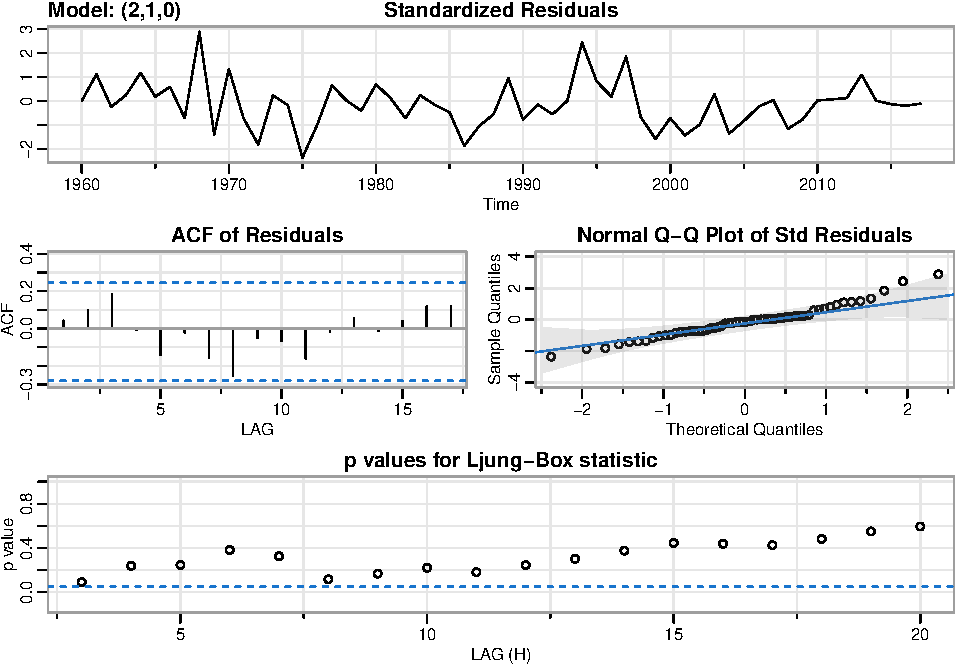
\includegraphics{STA_137_Final_Project_files/figure-latex/unnamed-chunk-10-1.pdf}

The Standardized Residuals plot shows that the mean of the residuals
seems to be 0 and the ACF and large p-values from the Ljung-Box test
indicate that the residuals are uncorrelated with each other. We can
assume that in this AR(2) model the residuals are a white noise process.

\begin{center}


\begin{tabular}{l|r|r}
\hline
  & MA\_1 & AR\_2\\
\hline
AIC & 4.841368 & 4.816436\\
\hline
BIC & 4.913055 & 4.923965\\
\hline
\end{tabular}

\end{center}

Finally let's look at the AIC and BIC for both of these models. Here we
want to consider which model has a lower AIC/BIC, but in this case there
is only a small difference between these values. Based on our residual
analysis and comparing the AIC/BIC for both models our final model is
the AR(2) or ARIMA(2,1,0) model since the residuals are a white noise
process. Our final model is defined in time series notation as:

\[y_t = (-0.5050) y_{t-1} + (-0.2897) y_{t-2} + w_t\]

\hypertarget{forecasting}{%
\subsubsection{Forecasting}\label{forecasting}}

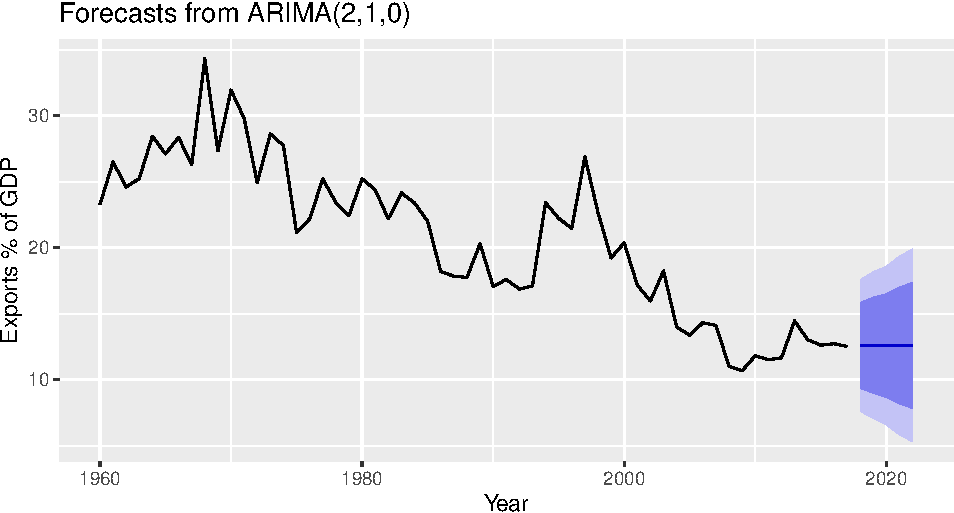
\includegraphics{STA_137_Final_Project_files/figure-latex/unnamed-chunk-12-1.pdf}

The above plot shows the forecast of C.A.R percentage of GDP from
exports over the next 5 years with the dark blue region as the 80\%
confidence region and the light blue region as the 95\% confidence
region. We can see that with 95\% confidence C.A.R exports will be
between about 5 and 19 percent of its total GDP per year over the next 5
years.

\hypertarget{conclusion}{%
\subsubsection{Conclusion}\label{conclusion}}

In this time series analysis we studied the exports of the Central
African Republic one of the most underdeveloped nations on Earth. We
conducted an exploratory data analysis and found a general downward
trend in exports from 1960 to 2017 due to political unrest and lack of
financial backing. Then we analyzed the ACF and PACF for this export
data in order to get an idea of what models would fit best. We concluded
that either an MA(1) or AR(2) model would be worth exploring further. We
then created models that estimated their respective parameters and
conducted a residual analysis to see if the white noise process
assumption was satisfied. After considering the residual analysis and
looking at the AIC/BIC for both models we choose an AR(2) model because
its residuals most resembled a white noise process. Finally we plotted
and interpreted a five year forecast from our AR(2) model. Throughout
this analysis we witnessed first hand how political instability caused
by colonialism negatively affects the Central African Republic's economy
after the nation gained independence.

\hypertarget{code-appendix}{%
\subsubsection{Code Appendix}\label{code-appendix}}

\begin{Shaded}
\begin{Highlighting}[]
\FunctionTok{library}\NormalTok{(magrittr)}
\FunctionTok{library}\NormalTok{(forecast)}
\FunctionTok{library}\NormalTok{(astsa)}

\FunctionTok{rm}\NormalTok{(}\AttributeTok{list=}\FunctionTok{ls}\NormalTok{())}
\FunctionTok{setwd}\NormalTok{(}\FunctionTok{dirname}\NormalTok{(rstudioapi}\SpecialCharTok{::}\FunctionTok{getActiveDocumentContext}\NormalTok{()}\SpecialCharTok{$}\NormalTok{path))}

\DocumentationTok{\#\#\#\# Step 0: Data Prep \#\#\#\#}

\FunctionTok{load}\NormalTok{(}\FunctionTok{paste0}\NormalTok{(}\FunctionTok{getwd}\NormalTok{(),}\StringTok{"/finalproject.RData"}\NormalTok{))}
\NormalTok{export\_data }\OtherTok{\textless{}{-}} \FunctionTok{ts}\NormalTok{(finalPro\_data}\SpecialCharTok{$}\NormalTok{Exports,}\DecValTok{1960}\NormalTok{,}\DecValTok{2017}\NormalTok{)}

\DocumentationTok{\#\#\#\# Step 1: Plot Data Identify Outliers \#\#\#\#}

\CommentTok{\# No outliers, general downward trend. Not stationary}
\NormalTok{export\_data }\SpecialCharTok{\%\textgreater{}\%}\NormalTok{ plot}

\DocumentationTok{\#\#\#\# Step: 2 Transform Data \#\#\#\#}

\CommentTok{\# log helps data be more stationary but impact on ACF/PACF is small }
\CommentTok{\#export\_data \%\textless{}\textgreater{}\% log}
\CommentTok{\#export\_data \%\textless{}\textgreater{}\% sqrt}
\CommentTok{\#export\_data \textless{}{-} 1 / export\_data}
\CommentTok{\#export\_data \textless{}{-} export\_data\^{}2 }

\DocumentationTok{\#\#\#\# Step 3: Take Differences If Not Stationary \#\#\#\#}

\CommentTok{\# 1st order difference looks stationary}
\NormalTok{export\_data\_diff }\OtherTok{\textless{}{-}}\NormalTok{ export\_data }\SpecialCharTok{\%\textgreater{}\%}\NormalTok{ diff}
\NormalTok{export\_data\_diff }\SpecialCharTok{\%\textgreater{}\%}\NormalTok{ plot}

\CommentTok{\# mean is close to 0}
\NormalTok{export\_data\_diff }\SpecialCharTok{\%\textgreater{}\%}\NormalTok{ mean}

\DocumentationTok{\#\#\#\# Step 4: Examine ACF/PACF \#\#\#\#}

\CommentTok{\# ACF implies MA(1)}
\CommentTok{\# PACF implies AR(2)}

\NormalTok{export\_data\_diff }\SpecialCharTok{\%\textgreater{}\%}\NormalTok{ acf}
\NormalTok{export\_data\_diff }\SpecialCharTok{\%\textgreater{}\%}\NormalTok{ pacf}


\DocumentationTok{\#\#\#\# Step 5: Create Models \#\#\#\#}

\NormalTok{ma\_model }\OtherTok{\textless{}{-}} \FunctionTok{sarima}\NormalTok{(export\_data,}\DecValTok{0}\NormalTok{,}\DecValTok{1}\NormalTok{,}\DecValTok{1}\NormalTok{,}\AttributeTok{no.constant =} \ConstantTok{TRUE}\NormalTok{)}
\NormalTok{ar\_model\_2 }\OtherTok{\textless{}{-}} \FunctionTok{sarima}\NormalTok{(export\_data,}\DecValTok{2}\NormalTok{,}\DecValTok{1}\NormalTok{,}\DecValTok{0}\NormalTok{,}\AttributeTok{no.constant =} \ConstantTok{TRUE}\NormalTok{)}


\DocumentationTok{\#\#\#\# Step 6: Check Residuals Are White Noise \#\#\#\#}

\DocumentationTok{\#\#\#\# Step 7: Forecast \#\#\#\#}

\NormalTok{forcast\_model }\OtherTok{\textless{}{-}} \FunctionTok{arima}\NormalTok{(export\_data, }\AttributeTok{order =} \FunctionTok{c}\NormalTok{(}\DecValTok{2}\NormalTok{,}\DecValTok{1}\NormalTok{,}\DecValTok{0}\NormalTok{))}
\FunctionTok{forecast}\NormalTok{(forcast\_model,}\AttributeTok{h =} \DecValTok{5}\NormalTok{) }\SpecialCharTok{\%\textgreater{}\%}\NormalTok{ autoplot}
\end{Highlighting}
\end{Shaded}


\end{document}
